\section{Differential Dynamic Microscopy}\label{sec:DDMDis}
The measured datasets were evaluated using a provided matlab script, which first calculated the dynamic structure function $D(q,\Delta t)$ for exponential increasing time differences $\Delta t$. Therefore, the difference intensities 
\begin{equation}
    \Delta I(x,y,\Delta t) = I(x,y,t+\Delta t) - I(x,y,t)
\end{equation}
were transformed into the fourier space intensities $\Delta I(q_x,q_y,\Delta t)$ using a 2d fast fourier trasform algorithm. $D(q,\Delta t)$ is obtained by averiging radial over the dynamic structure function 
\begin{equation}
    D(q_x,q_y,\Delta t) = \langle |\Delta I(x,y,\Delta t)|^2 \rangle.
\end{equation}
Resulting plots of $D(q_x,q_y,\Delta t)$ for selected $q$ can be seen in fig.~\ref{fig:DvsDeltat}. Hereby can be seen, that especially for small $q$ increasing $\Delta t$ lead to bigger noise and poor statistics. Therefore, a cutoff for $\Delta t$ was set manually. \par 

\begin{figure}[ht]
    \centering
    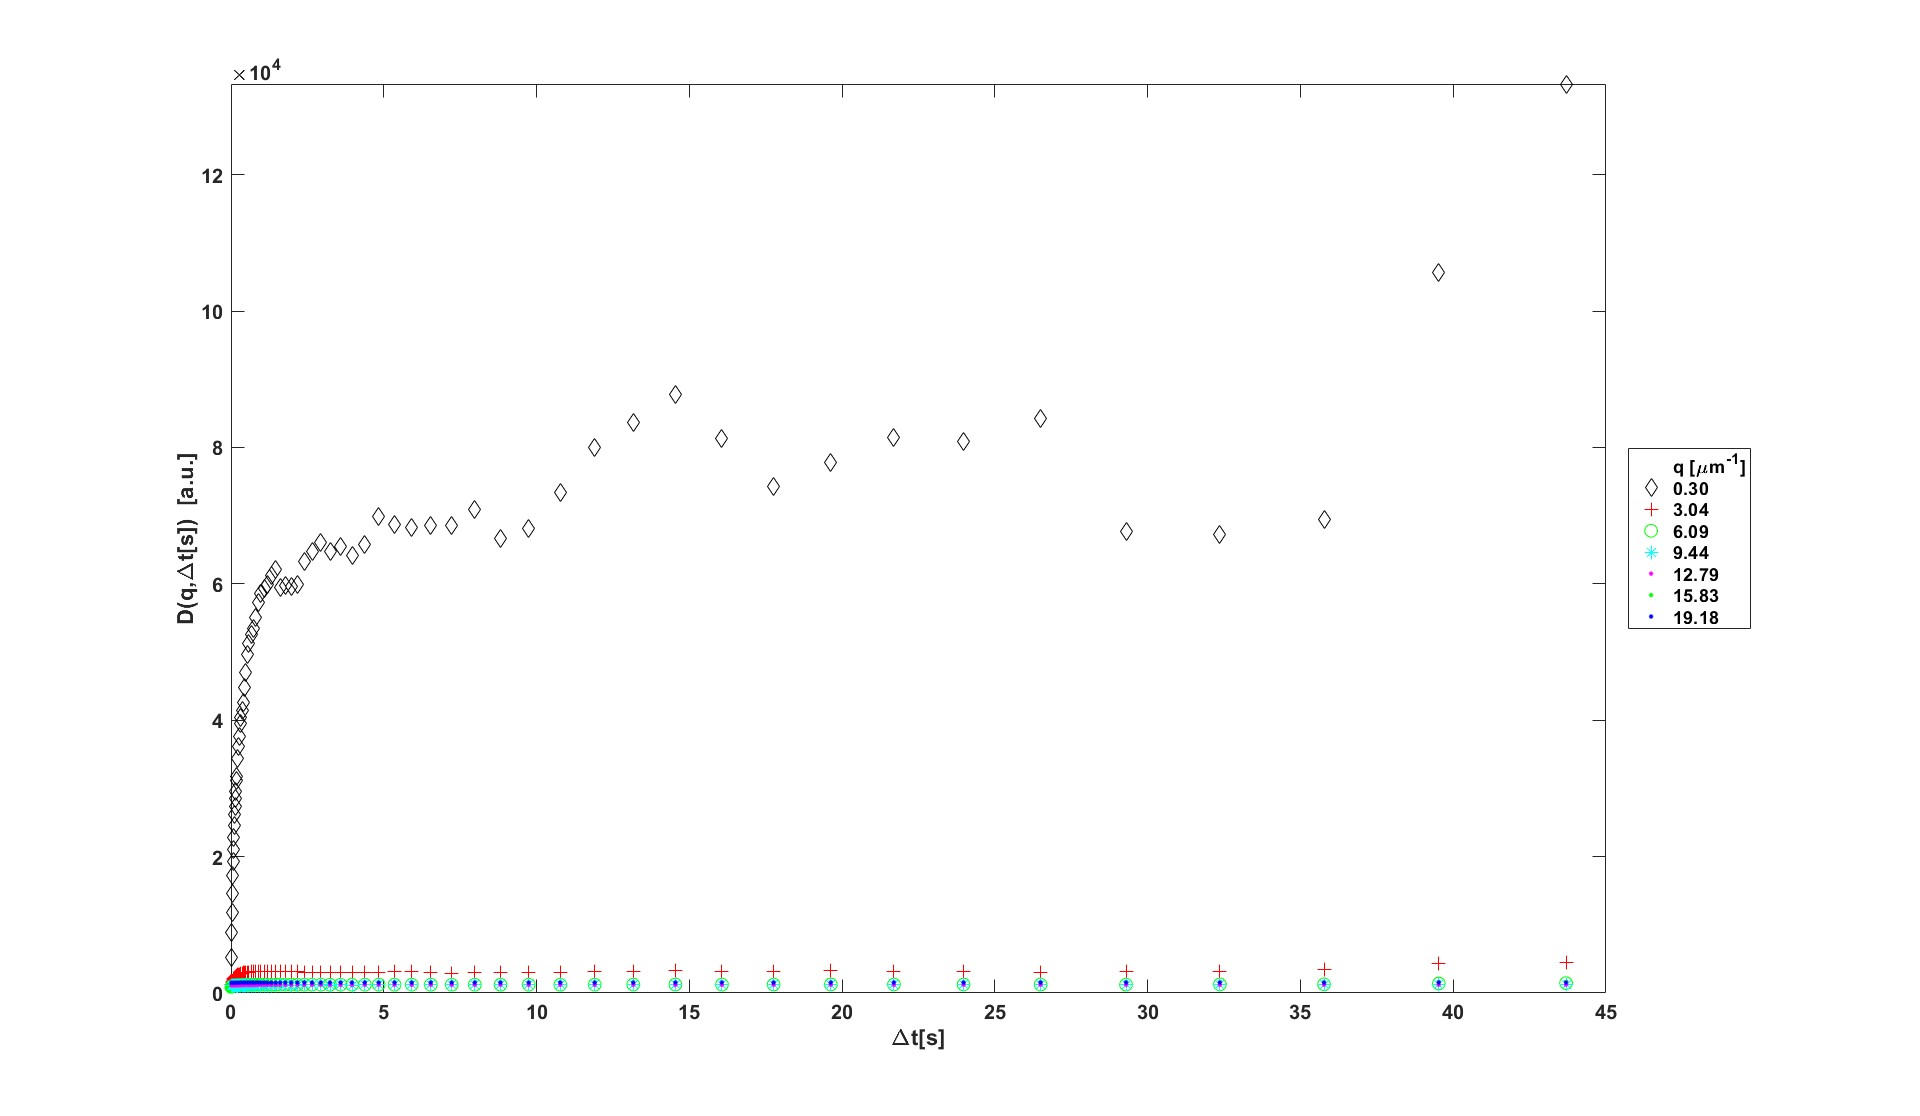
\includegraphics[width = \textwidth]{Bilder/Auswertung/DDM/d vs detat.jpg}
    \caption{The calculated dynamic structure function $D(q_x,q_y,\Delta t)$ is plotted against $\Delta t$ for selected $q$. For small $q$ an increasing $\Delta t$ leads to bigger noise and poor statistics.}
    \label{fig:DvsDeltat}
\end{figure}

As the dynamic structure function is expected to follow eq.~\ref{eq:21.3}, a fit was made, obtaining $A(q)$, $B(q)$ and $\tau (q)$. Eq.~\ref{eq:21.4} states 
\begin{equation}
    \tau (q) \propto q^{-2}
\end{equation}
and therefore the log-log-plot of $\tau (q)$ against $q$ should be a straight line with slope \num{-2}. As can be seen in fig.~\ref{fig:tauvsQ}, this is not the case for too small or too big $q$. Consequently a range for $q$ for the application of the fit of eq.~\ref{eq:21.4} was set. In this way, for each dataset a value for $D_m$ was obtained. As for every configuration of the setup five measurements were done, the $D_m$ were averaged afterwards. The results are stated in tab.~\ref{tab:Dm}.

\begin{figure}[ht]
    \centering
    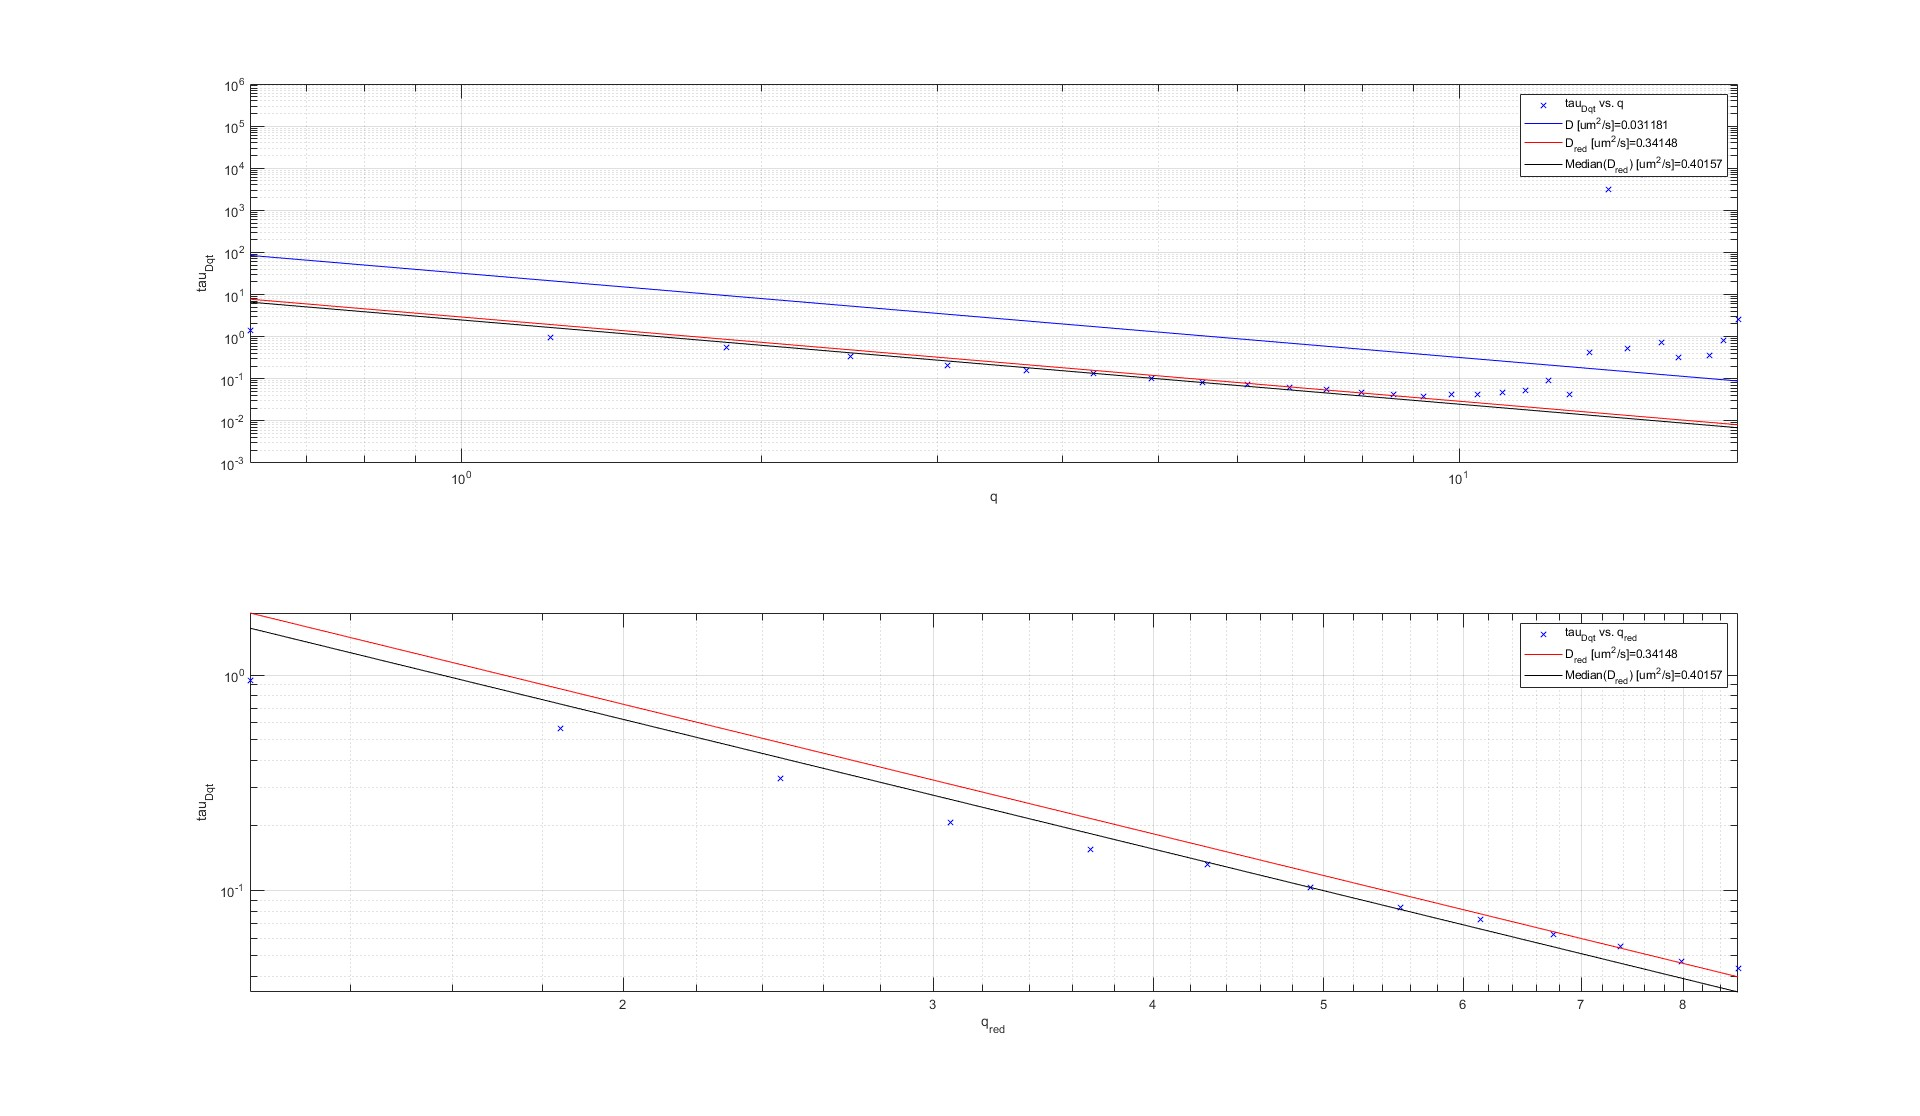
\includegraphics[width = \textwidth]{Bilder/Auswertung/DDM/tauvsQ.jpg}
    \caption{The values for $\tau (q)$ obtained from the fits were plotted against $q$ (upper plot). Too small and too big $q$ do not follow eq.~\ref{eq:21.4} and therefore lead to a wrong value for $D_m$ (fit in blue). Cosequently, the fit is only applied to a manually defined reduced $q$ space (lower plot and fits in red and black).}
    \label{fig:tauvsQ}
\end{figure}

\begin{table}
    \centering
    \begin{tabular}{c c c | c c}
        \toprule
        binning & ROI size / px & pinhole & $D_m$ / \si{\micro\meter^2 \per\second} & range for $q$ / \si{\per\micro\meter}\\
        \midrule
        none & 256x256 & none & \num{1.7 \pm 0.4} & 1-4\\
        none & 256x256 & half open & \num{1.7 \pm 0.7} & 1-3\\
        none & 256x256 & closed & \num{1.6 \pm 0.4} & 1-4\\
        \midrule
        none & 128x128 & none & \num{1.8 \pm 0.6} & 1-3.5\\
        none & 128x128 & half open & \num{1.7 \pm 0.9} & 1-4\\
        none & 128x128 & closed & \num{2.2 \pm 0.2} & 1-4\\
        \midrule
        2x2 & 128x128 & none & \num{0.56 \pm 0.10} & 1-8\\
        2x2 & 128x128 & half open & \num{0.86 \pm 0.11} & 1-5\\
        2x2 & 128x128 & closed & \num{0.49 \pm 0.12} & 1-9\\
        \midrule
        2x2 & 64x64 & none & \num{0.63 \pm 0.15} & 1-7\\
        2x2 & 64x64 & half open & \num{0.7 \pm 0.3} & 1-5\\
        2x2 & 64x64 & closed & \num{0.55 \pm 0.09} & 1-7.5\\
        \midrule
        4x4 & 64x64 & none & \num{0.15 \pm 0.03} & 4-10\\
        4x4 & 64x64 & half open & \num{0.15 \pm 0.03} & 3.5-10\\
        4x4 & 64x64 & closed & \num{0.11 \pm 0.03} & 3-10\\
        \bottomrule
    \end{tabular}
    \caption{Calculated averaged values of $D_m$ for each setting. The selected range of $q$ can differ slightly throughout the single measurements of a setup. }
    \label{tab:Dm}
\end{table}

When looking at the selected $q$ ranges, it can be seen that for the 4x4 binning the resolution for small $q$ gets worse in comparison to smaller binning. This fulfills our expectations since due to the binning, more pixels are summarized to one. Therefore, the minimum evaluation length in our ROI increases and the resolution for small $q$ decreases (see also sec.~\ref{sec:qSpace}). However, we would also expect a smaller resolution for big $q$ with an decreasing ROI size, following the same argument. This we could not observe. In fact, the resoultion even increases and is best for the smallest ROI size (64x64 px). This might be due to a better measuring procedure after having done some measurements already. \\
We also observe in general smaller uncertainties and better fits for the closed aperture. This is expectable, since ,as shown in sec.~\ref{sec:LightSheet}, the thickness of the lightsheet decreases with the beam diameter. \\
Within a certain setup, the calculated values are more or less the same within the uncertainties. However, a change in setup leads to a different obtained $D_m$ value. This is suprising, since the probe did not change. Therefore, we assume, that binning and the ROI size has an effect on the measurement quality. To verify our calculated values, the theoretical value shall be estimated. As we are at diffusie timescales, the Stokes Einstein equation can be used, which proposes a diffusion constant of 
\begin{equation}
    D_{SE} = \frac{k_BT}{6 \pi \eta R_0}
\end{equation}
with the dynamic viscosity $\eta$ and the radius of the particle $R_0$. $\eta$ of the \SI{1}{\percent}wt agarose solution depends on various parameters, such as temperature, solvent properties etc. However, for our estimation, we assume $\eta = $\SI{0.01}{\pascal\second}. Further, in this experiment, $T=$\SI{300}{\kelvin} and $R_0=$\SI{100}{\nano\meter}. This leads to a theoretical value of 
\begin{equation}
    D_{SE} = \SI{0.22}{\micro\meter^2 \per\second}.
\end{equation}

This value corresponds best to the values with the maximum binning and the minimum ROI size in our measurement. This is surpising since we expect binning to decrease the measurement accuracy because the information of several pixels get summarized in only a single one, especially since the pixelsize is $d_{px} = $\SI{162.5}{\nano\meter} and therefore in the size range of the particles themselves. Additional binning therefore should not be able to sufficiently track the diffusion of the particles. Also the decrease in measurement area should lead to a maximum equal good result, since less information is gathered. The simplifications made (no flow present, 2d analysis of 3d diffusion) shlould not be an explanation for this discrepancy since those all overestimate the diffusion and therefore corrections would only increase the difference between expected and calculated values. We hence suppose that the error might be in the estimation of the theoretical value of $D_{SE}$ as especially the value for $\eta$ is quite uncertain, $D_{SE}$ may also vary in one order of magnitude which would lead to a support of the values of the non binned, big ROI sized setup.